\label{sec:intro}
% \paragraph{Real-world problem scenario}
According to World Health Organisation (WHO) \cite{who2025cvd}, cardiovascular disease (CVDs)
is one of the urgent and primary cause of global deaths. It was estimated 19.8 milion people died from CVDs, accounting for roughly 32\% of all reported deaths globally,
and approximately 85\% were diagnosed with strokes and heart attacks. Over three quarters of CVD-related deaths were reported in low– to middle–income nations.
Evidently, during 1990 and 2022, as surveyed by \cite{LINDSTROM20222372, martin2025heart}, the mortality rate due to CVDs witnessed significant drops; however, in developing countries, improvement were gained but insignificant, e.g. Central Latin America, South East Asia, North Africa and Middle East.
Even worse, South Asia and almost African nations suffered from the rise of CVDs-diagnosed deaths.

Besides maintaining a healthy lifestyle by managing behavioural and environmental risk factors, e.g. tobacco use, alcohol consumption, excessive use of salt, sugar and fats, physical inactivity and air pollution \cite{whf2023, who2025world}.
It is of highly demanding to develop early symptomps of CVDs detectors, so that medical inference can begin as early as possible to mitigate the adverse impacts \cite{who2025cvd}.
Several medical statistics can be leveraged to conduct health diagnosis, e.g.  phonocardiogram (PCG) \cite{shuvo2021cardioxnet}, photoplethysmography (PPG) \cite{simonyan2021spectral}, invasive techniques (i.e. implanting biosensors to patients' body) \cite{CTC4CVD}, clinical, demographic features and physical examinations \cite{nikam2020cardiovascular, qian2022cardiovascular, rahim2021integrated, yang2023predicting, akkaya2022comparative, chicco2021machine, ghorashi2023leveraging, joo2020clinical}.
Nonetheless, in this article, we shall discuss applications of machine learning techniques for CVD early detection using Electrocardiography (ECG), which is a non–invasive and cost-effective tool \cite{sinha2023dasmcc, siontis2021ai, strodthoff2021ptbxl}. 
Before reviewing state–of–the–art (SOTA) approaches and results, let us offer some background knowledge about ECG below, fully adopted from \cite{GOLDBERGER2018xi}, which are essentially important to extract meaningful features for modelling pipeline.

The electrocardiogram or electrocardiography (ECG or EKG) is a time–series visualisation of cardiac electrical activity, offering the so–called ``time–voltage chart of the heartbeat''.
ECGs can be produced by attaching sensors, also known as electrodes, on different body parts, to record cardiac electrical currents. In practices, different number of locations are chosen, which produce different types of what–called ECG Leads.
In this work, we shall consider the 12–lead ECG, which is believed as the gold standard for clinical practices, though smaller number of leads, e.g. single–lead and three–lead, can be used and were studied in \cite{witvliet2021handheld, rajakariar2020smartwatch, hernandez2023threelead}.
An illustration of electrode placements for a standard 12–lead ECG is shown as follows.

\begin{figure}[H]
    \centering
    \begin{subfigure}[b]{0.45\textwidth}
        \centering
        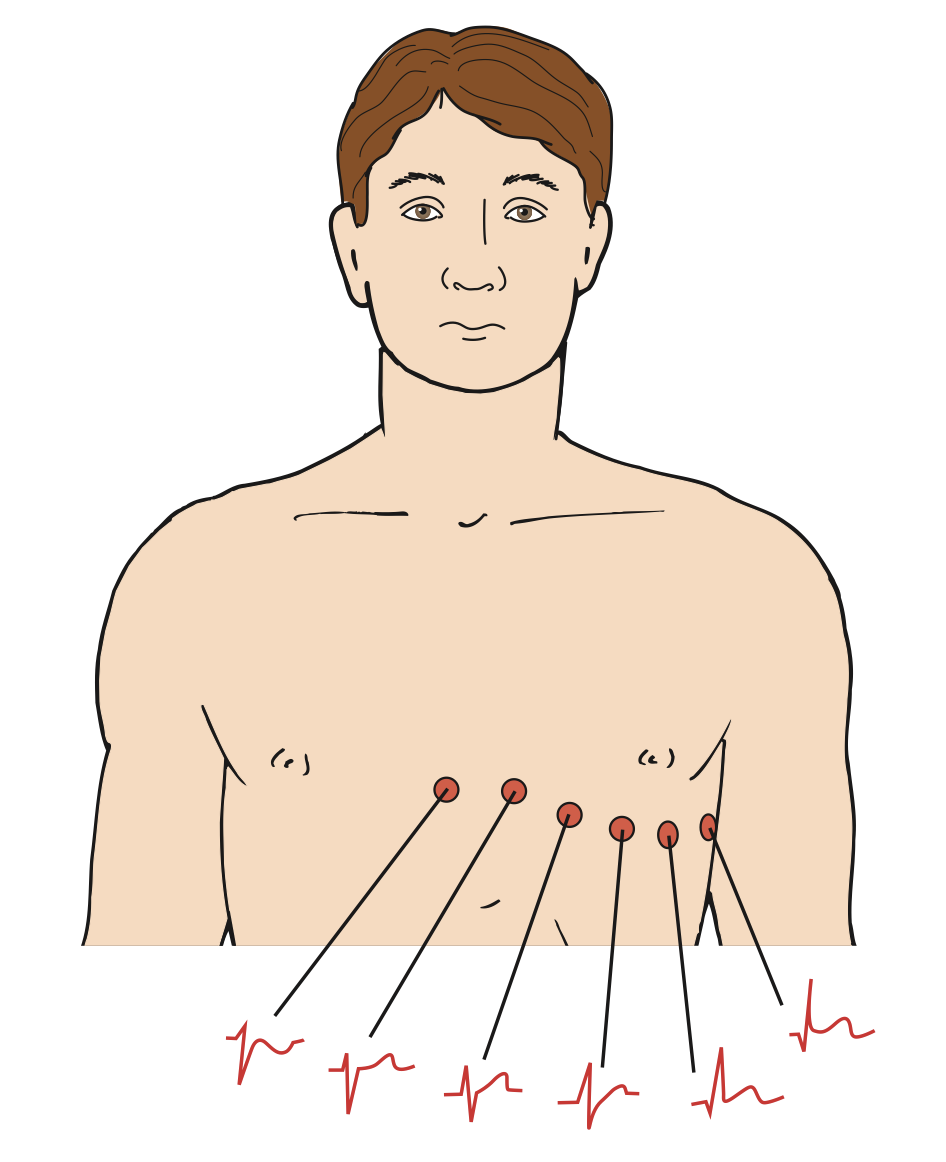
\includegraphics[height=6cm]{figures/intro_eda/chest_electrodes.png}
        \caption{Chest (precordial) electrodes.}
        \label{fig:chest-electrodes}
    \end{subfigure}
    \hfill
    \begin{subfigure}[b]{0.45\textwidth}
        \centering
        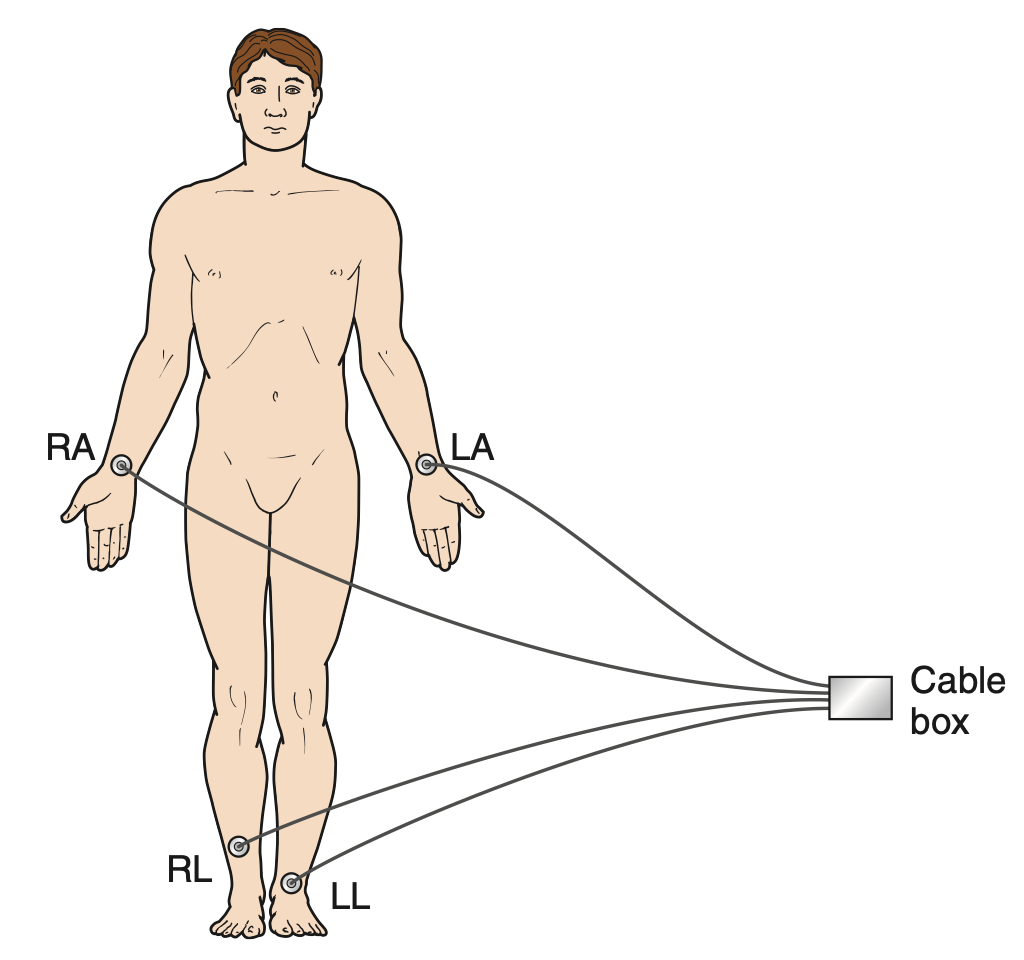
\includegraphics[height=6cm]{figures/intro_eda/body_electrodes.png}
        \caption{Limb electrodes.}
        \label{fig:body-electrodes}
    \end{subfigure}
    \caption{Electrode placement for a standard 12–lead ECG recording, adopted from \cite{GOLDBERGER2018xi}.
    (a) The six chest electrodes $V_1$–$V_6$.
    (b) The four limb electrodes: right arm (RA), left arm (LA), left leg (LL) and right leg (RL).}
    \label{fig:ecg-electrodes}
\end{figure}


The 12 leads are: $V_1$–$V_6$ + Lead I, II, III + aVR, aVL, aVF, where \cite{GOLDBERGER2018xi, doi:10.1161/CIRCULATIONAHA.106.180201} define:
\begin{equation}
    \label{eq:12lead}
    \begin{alignedat}{3}
        \text{Lead I} &= \text{LA} - \text{RA},
        &\quad \text{Lead II} &= \text{LL} - \text{RA},
        &\quad \text{Lead III} &= \text{LL} - \text{LA}, \\[4pt]
        \text{aVR} &= -\frac{\text{Lead I} + \text{Lead II}}{2},
        &\quad \text{aVF} &= \frac{\text{Lead II} + \text{Lead III}}{2},
        &\quad \text{aVL} &= -(\text{aVR} + \text{aVF}).
    \end{alignedat}
\end{equation}

Since the ECG is a time–voltage chart, it is a wave–like charts, comprising of different waveforms, which we shall introduce next.

\begin{figure}[H]
    \centering
    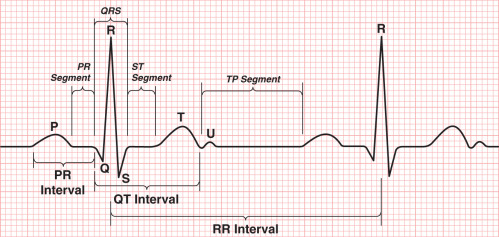
\includegraphics[width=1\textwidth]{figures/intro_eda/comprehensive_ecg.png}
    \caption{The characteristic waveforms, segments and intervals of a single cardiac cycle on an ECG trace, adopted from \cite{GOLDBERGER2018xi}.
    The P wave, the QRS complex, and the T wave, occasionally followed by a small U wave.
    The PR and QT intervals, the PR, ST and TP segments, and the RR interval are the timing measurements most commonly used in clinical interpretation.}
    \label{fig:ecg-waveform}
\end{figure}

The \texttt{PTB-XL} dataset consists of 12 temporal waveform charts representing 12 above–mentioned leads, each of which is characterised by the peaks, intervals and segments as demonstrated, further details will be presented in \textbf{Sec. \ref{sec:dataset}}.


Due to its abundant source of informative signals yet demanding advanced expertise to comprehend and ubdoubtedly subtle patterns may be missed by doctors, AI–based systems has become considerably important to detect patterns in ECGs \cite{siontis2021ai}.


% \paragraph{Recent solutions and results}
Automated ECG interpretation has progressed through two broad phases.
Classical pipelines first delineate the waveform of \textbf{Fig. \ref{fig:ecg-waveform}}, extract hand–crafted descriptors, i.e. wave amplitudes, PR/QT/RR durations, heart–rate variability statistics and spectral or wavelet coefficients, and pass them to shallow classifiers such as support vector machines, random forests or gradient–boosted trees.
The DASMcC classifier in\cite{sinha2023dasmcc}, which this report reproduces, is a recent representative of this family, it augments an imbalanced multi–class dataset using SMOTE before training tree–based ensembles on time–series features.
Such pipelines remain attractive because their inputs are clinically interpretable and their computational footprint is modest.

The prevailing SOTA, by contrast, applies end–to–end deep learning directly to the raw sampled waveform, dispensing with explicit feature engineering.
\cite{hannun2019cardiologist} trained a $34$–layer \texttt{ResNet} on more than $90{,}000$ single–lead ambulatory recordings and matched or exceeded an averaged cardiologist committee across twelve rhythm classes.
After that, \cite{ribeiro2020automatic} scaled the approach to 12–lead data, training on over two million exams from a Brazilian telehealth network and reporting $F_1$ scores above $80\%$ at specificity above $99\%$ for six abnormality classes.
Deep models can moreover surface conditions that are not visually apparent to a human reader, e.g. \cite{attia2019screening} identified asymptomatic left–ventricular systolic dysfunction from a standard 12–lead trace with an AUC near $0.93$, a capability surveyed more broadly by \cite{siontis2021ai}.

Because these headline results rest on private institutional cohorts, they are difficult to compare directly.
The release of \texttt{PTB-XL} \cite{wagner2020ptbxl} supplied a large, public, multi–label benchmark.
The accompanying study \cite{strodthoff2021ptbxl} established modern \texttt{1D–CNN} architectures of the \texttt{ResNet} and \texttt{Inception} families attain a macro–averaged AUC of roughly $0.93$ and consistently outperform recurrent and feature–based baselines, a ranking corroborated by \cite{smigiel2021ecg}.

The gap DASMcC targets is therefore one of deployability rather than raw accuracy.
\cite{sinha2023dasmcc} argued that models trained end–to–end on millions of raw traces are too heavy for IoT–based smart healthcare framework, and offer instead a lightweight, real–time classifier driven by only sixteen time–domain features of the 12–lead signal.

The contributions of this report are:
\begin{itemize}
    \item Critical analysis of the presented \cite{sinha2023dasmcc} vs. reproduced results.
    \item Proposal of our ML solution to the research problem being discussed.
    \item Empirical benchmark on the effect of dimensionality in ML classifiers.
\end{itemize}
Throughout this report, we shall refer to \cite{sinha2023dasmcc}, which is the paper we are attempting to reproduce, as original paper.

The remainder of this report is organised as follows. In \textbf{Sec. \ref{sec:dataset}}, we conduct an Exploratory Data Analysis (EDA) on \texttt{PTB–XL} dataset.
\hyperref[sec:part_1]{\textbf{Part 1}} presents approach and the reproduced results, along with certain critical reflections on any discrepancies identified between our and their results.
\hyperref[sec:part_2]{\textbf{Part 2}} is based on the evidence in the prior part, we argue and propose another ML solution and benchmark against their results.
% This report reproduces those claims, and then asks whether the reported margin survives augmentation applied within rather than before cross–validation \cite{demircioglu2024oversampling}, as examined in \textbf{Part 1}.
